%%%%%%
%
% PROJECT 10 - SARS
%
% filename: SARS.tex
% last modified: 2014-1-24
%
%%%%%%%
%
% IN THIS PROJECT, STUDENTS STUDY THE SIR MODEL AND HOW IT APPLIES TO
% THE SPREAD OF SARS IN 2003 IN ASIAN AND CANADA.
%
% HUGHES-HALLET P. 634
%
%%%%%%%

\documentclass
[justified,nohyper]
{tufte-handout}

\usepackage{amsmath}


\usepackage{booktabs}
\usepackage{graphicx}
\usepackage{kmath,kerkis} % The order of the packages matters; kmath changes the default text font
\usepackage[T1]{fontenc}

\begin{document}
\section{Advanced Calculus Project 10: SARS}

\newthought{In the spring of 2003}, SARS (Severe Acute Respiratory Syndrome) spread rapidly in several Asian countries and Canada. Predicting the course of the disease -- how many people would be infected, how long it would last -- was important to officials trying to minimize the impact of the disease.

As prepartion for this project, please read the article\sidenote{\url{http://goo.gl/YHo9wu}} published in the \textit{Journal of The Royal Society of Medicine}. It is a summary of what happened and some of the lessons learned. If you have trouble accessing the article, please email me\sidenote{\url{eabell@sasaustin.org}} or talk with me in class.

In part 1 of this project, you will compare three predictions about the spread of SARS in Hong Kong. In part 2, you will develop a more sophisticated SIR-model and investigate the effectiveness of a quarantine policy.

\section{Part 1: Three Predictions}
We measure time, $t$, in days since March 17, 2003, the date the World Health Organization (WHO) started to publish daily SARS reports.\sidenote{\url{http://goo.gl/t4d9dp}} Let $P$ be the total number of cases reported in Hong Kong by day $t$. On March 17, Hong Kong reported 95 cases. The constants in the three differential equations whose predictions are analyzed in this project were determined using WHO data available March 2003. We compare predictions from the three models for June 12, 2003, the last day a new case was reported in Hong Kong.

\begin{enumerate}
  \item A Linear Model. Suppose $P$ satisfies
  \[
      \dfrac{dP}{dt} = 30.2, \qquad \text{ with }  P(0)=95
  \]
  Solve the differential equation and use your solution to predict the number of cases of SARS in Hong Kong by June 12 ($t=87$).
  
  \item An Exponential Model. Suppose $P$ satisfies
  \[
      \dfrac{1}{P}\dfrac{dP}{dt} = 0.12, \qquad \text{with } P(0)=95
  \]
  Solve the differential equation and use your solution to predict the number of cases of SARS in Hong Kong by June 12 ($t=87$).
  
  \item A Logistic Model. Suppose $P$ satisfies
  \[
      \dfrac{1}{P}\dfrac{dP}{dt} = 0.19 - 0.0002P, \qquad \text{with } P(0)=95
  \]
  Solve the differential equation and use your solution to predict the number of cases of SARS in Hong Kong by June 12 ($t=87$).
\end{enumerate}

After solving each of the three models, answer the following questions in your report.

\begin{enumerate}
  \item Comment on the June 12 predictions from the three models. How do they compare? How would you justify one model over the other two? Pretend like you are doing this just after March 17 and you are responsible for informing the world what will happen.
  \item What do each of the three models predict about the trend in the number of new cases each day?
  \item In May 2003, the \textit{Journal of The Royal Society of Medicine} published a graph shown in Figure \ref{dailyinc}. What trend do you see in the data? What does this trend suggest about which model fits the data best?


  \item Assuming that the data follow a logistic model, which is the only one of the three models to predict that the total number of cases will level off, complete the following two analysis steps.
  \begin{enumerate}
  \item Use $P(t)$ from the logistic model solution to predict the maximum number of SARS cases.
  \item Assume that the data follow a logistic model, but not necessarily with the parameters given previously. Use Figure \ref{dailyinc} and the fact that there had been a total of 998 cases of SARS by April 10 to develop a new $P(t)$ solution and use it to predict the maximum number of SARS cases.
\end{enumerate}

  \item To see how well the three models worked in practice, plot the data in Table \ref{sarscases} and each of your solution curves for the three models. Be sure to label each curve with an appropriate legend and scaled axes.
\end{enumerate}


\begin{fullwidth}
\begin{table}
\begin{tabular}{cccccccc}
    \toprule
    $t$ & $P$ & $t$ & $P$ & $t$ & $P$ & $t$ & $P$ \\
    \cmidrule(r){1-2}\cmidrule(r){3-4}\cmidrule(r){5-6}\cmidrule{7-8}
    0 & 95 & 26 & 1108 & 54 & 1674 & 75 & 1739 \\
    5 & 222 & 33 & 1358 & 61 & 1710 & 81 & 1750 \\
    12 & 470 & 40 & 1527 & 68 & 1724 & 87 & 1755 \\
    19 & 800 & 47 & 1621 & & &  \\
    \bottomrule
\caption{\label{sarscases} Total number of SARS cases reported in Hong Kong by day $t$ (where $t=0$ is March 17, 2003)}
\end{tabular}
\end{table}
\end{fullwidth}

\begin{figure}
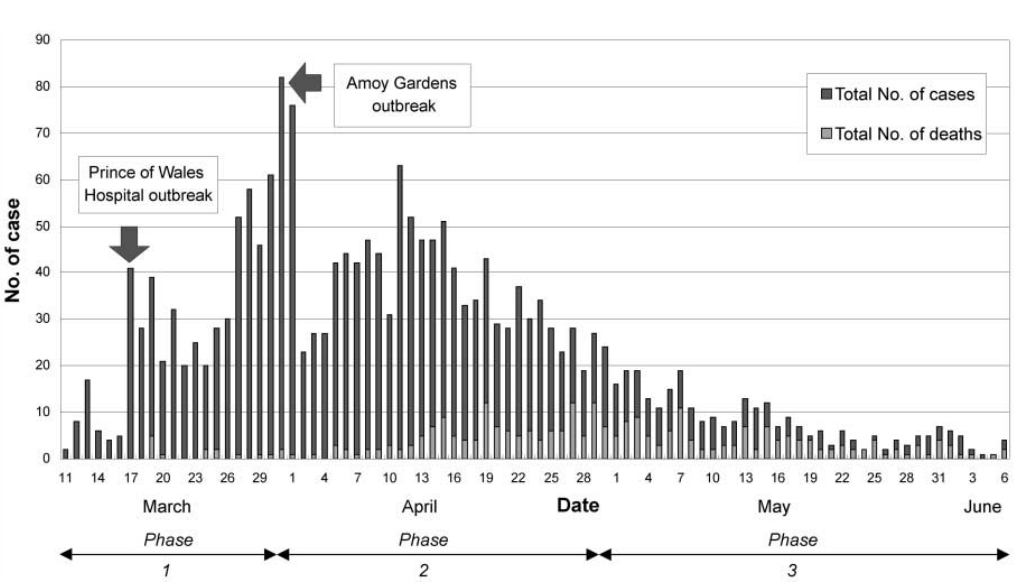
\includegraphics[scale=0.3]{dailyincrease.png}
\caption{\label{dailyinc} Daily increase in Hong Kong SARS cases, \url{http://goo.gl/YHo9wu}}
\end{figure}

\newpage

\section{Part 2: An SIR Model}
As we have seen, a possibly better and more accurate way of modeling the spread of a disease is to use an SIR model. In this part of the project, you will develop a SIR model for the spread of SARS.

The variables are $S$, the number of susceptibles, $I$, the number of infecteds who can infect others, and $R$, the number removed (this group includes those in quarantine and those who die, as well as those who have recovered and aquired immunity). Time, $t$, is in days since March 17, 2003, the date the World Health Organization started to publish daily SARS reports.

In this model,
\begin{align*}
    \frac{dS}{dt} &= -aSI \\
    \frac{dI}{dt} &= aSI - bI
\end{align*}

and $S+I+R = 6.8$ million, the population of Hong Kong in 2003. \sidenote{\url{www.census.gov}, International Data Base (IDB)} Estimates based on WHO data give $a=1.25\cdot 10^{-8}$.

\begin{enumerate}
  \item What are $S_0$ and $I_0$, the initial values of $S$ and $I$?
  \item During March 2003, the value of $b$ was about 0.06. Plot the slope field for this system of differential equations and the solution trajectory corresponding to the initial conditions. Use \[0\leq S \leq 7\cdot 10^{6},\quad 0\leq I \leq 0.4\cdot 10^{6}\]
  \item What does your graph tell you about the total number of people infected over the course of the disease if $b=0.06$? What is the threshold value? What does this value tell you?
  \item During April, as public health officials worked to get the disease under control, people who had been in contact with the disease were quarantined. Explain why quarantining has the effect of raising the value of $b$.
  \item Using the April value, $b=0.24$, plot the slope field. (Use the same value of $a$ and the same axes size so that you can easily compare with the previous slope field.)
  \item What is the threshold value for $b=0.24$? What does this tell you? Comment on the quarantine policy.
  \item Comment on the effectiveness of each of the following policies intended to prevent an epidemic and protect a city from an outbreak of SARS in a nearby region. Would either of these be useful precautions to take? Explain.
  \begin{enumerate}
  \item Close off the city from contact with the infected region. Shut down roads, airports, trains, and other forms of direct contact.
  \item Install a quarantine policy. Isolate anyone who has been in contact with a SARS patient or anyone who shows symptoms of SARS.
\end{enumerate}

Conclude your report by summarizing your experience working on this project. What you have done is essentially what an epidemiologist would do in analyzing the spread of an infectious disease by developing several models and comparing their effectiveness. You have utilized Calculus as a powerful and effective tool. The decisions made based on this kind of work can have significant and far-reaching impact.

\end{enumerate}



\end{document}